\documentclass[12pt]{article}
\usepackage{longtable}
\usepackage{geometry}
\geometry{left=1.25 in,right=1.25 in,top=1.00in,bottom=1.0in}

%\documentclass[justified,notoc]{tufte-handout2}
%need to figure out why figure refernces are messed up

\usepackage{natbib}   % call natbib
\setcitestyle{authoryear}  % set citation style to authoryear
\bibliographystyle{plainnat} % use the plainnat instead of plain
\usepackage{booktabs}
\usepackage{amssymb, amsmath, amsfonts}
\usepackage{outlines}
\usepackage{soul}
\usepackage[gen]{eurosym}
\usepackage{graphicx}

\usepackage{fancyhdr}
\usepackage{authblk}
\usepackage{lineno}
\usepackage[hyphens]{url}
\usepackage{hyperref}
\hypersetup{
 colorlinks = true, %Colours links instead of ugly boxes
 urlcolor  = blue, %Colour for external hyperlinks
 linkcolor = blue, %Colour of internal links
 citecolor = blue %Colour of citations
}
\pagestyle{fancy}
\usepackage{outlines}
\usepackage{caption}
%\captionsetup[table]{name=Figure}
\graphicspath{{../input/}}
\usepackage[outdir=./]{epstopdf}


\usepackage{enumitem}
\setlist[enumerate,2]{label=\roman*)}
\setlist[enumerate,3]{label=\Roman*)}
\setlist[enumerate,4]{label=\roman*)}

%\renewcommand{\familydefault}{\sfdefault}
% ------------------------------- use \citep{FAQs} to cite
\usepackage{filecontents}
\begin{filecontents}{\jobname.bib}
}

@article{Ross2016a,
  title   = {{The Supervisory Capital Assessment Program}},
  publisher = "Yale Program on Financial Stability",
  author  = "Ross, Chase P.",
  year   = "2016",
  doi    = " ",
  volume  = " ",
  journal  = "Yale Program on Financial Stability Intervention Case",
  issn   = " ",
  url    = {http://papers.ssrn.com/sol3/papers.cfm?abstract_id=2722712},
}

@article{Ross2016b,
  title   = {{Financial Services Authority 2008/9 Stress Tests}},
  publisher = "Yale Program on Financial Stability",
  author  = "Ross, Chase P.",
  year   = "2016",
  doi    = " ",
  volume  = " ",
  journal  = "Yale Program on Financial Stability Intervention Case",
  issn   = " ",
  url    = {http://som.yale.edu/download-ypfs/Financial-Services-Authority-Tests.pdf},
}

@article{RossWiggins,
  title   = {{European Central Bank Tools and Policy Actions A: Open Market Operations, Collateral Expansion and Standing Facilities}},
  publisher = "Yale Program on Financial Stability",
  author  = "Ross, Chase P., and Wiggins, R. and Metrick, A.",
  year   = "2016",
  doi    = " ",
  volume  = " ",
  journal  = "Yale Program on Financial Stability Intervention Case",
  issn   = " ",
  url    = {http://papers.ssrn.com/sol3/papers.cfm?abstract_id=2721873},
}

@article{Sunderji,
  title   = {{European Bank Stress Test Results: A Systemic Positive, Despite the Oversights}},
  publisher = "Barclays Capital",
  author  = "Sunderji, Aziz, and Julius, Jeroen, and Leeming, Matt",
  year   = "2010",
  doi    = " ",
  volume  = " ",
  journal  = "Barclays Capital Credit Research",
  issn   = " ",
}

@article{Samuels,
  title   = {{Happy Now? Four Questions on the European Banks' Stress Test}},
  publisher = "Barclays Capital",
  author  = "Samuels, Simon and Harrison, Mike",
  year   = "2010",
  doi    = " ",
  volume  = " ",
  journal  = "Barclays Capital Credit Research",
  issn   = " ",
}


@article{Deutsche,
  title   = {{Interpreting the Stress Test Results}},
  publisher = "Deutsche Bank",
  author  = "Spick, Matt",
  year   = "2010",
  doi    = " ",
  volume  = " ",
  journal  = "Deustche Bank European Bank Strategy",
  issn   = " ",
}

@article{Goldman,
  title   = {{European Weekly Analyst, Issue No. 10/27: On the Eve of the Bank Stress Tests}},
  publisher = "Goldman, Sachs Global Investment Research",
  author  = "Kojucharov, Nick",
  year   = "2010",
  doi    = " ",
  volume  = " ",
  journal  = "Goldman Sachs Global Investment Research",
  issn   = " ",
}


@article{CEBS2009,
  title   = {{Press Release: 2981st Council Meeting, Economic and Financial Affairs}},
  publisher = "Council of the European Union",
  author  = {{Council of the European Union}},
  year   = "2009",
  doi    = " ",
  volume  = " ",
  journal  = " ",
  issn   = " ",
  url    = {https://www.consilium.europa.eu/uedocs/cms_data/docs/pressdata/en/ecofin/111706.pdf},
}


@article{Methodology,
  title   = {{Aggregate Outcome of the 2010 EU Wide Stress Test Exercise Coordinated by CEBS in Cooperation with the ECB}},
  publisher = "Committee of European Banking Supervisors",
  author  = {{Committee of European Banking Supervisors}},
  year   = "2010",
  doi    = " ",
  volume  = " ",
  journal  = " ",
  issn   = " ",
  url    = {https://www.eba.europa.eu/documents/10180/15938/Summaryreport.pdf/95030af2-7b52-4530-afe1-f067a895d163},
}

@article{Gonzalez,
  title   = {{Spanish Financials: Interpreting the Stress Test Results: Banks and Cajas}},
  publisher = "Deutsche Bank",
  author  = "Gonzalez, Carlos Berastain",
  year   = "2010",
  doi    = " ",
  volume  = " ",
  journal  = "Deustche Bank Global Markets Research",
  issn   = " ",
}

@article{SCAPResults,
  title   = {{The Supervisory Capital Assessment Program: Overview of Results}},
  publisher = "Board of Governors of the Federal Reserve System",
  author  = {{Federal Reserve}},
  year   = "2009",
  doi    = " ",
  volume  = " ",
  journal  = " ",
  issn   = " ",
  url    = {http://www.federalreserve.gov/newsevents/press/bcreg/bcreg20090507a1.pdf},
}

@article{SG,
  title   = {{European Bank Stress Tests}},
  publisher = "Societe Generale",
  author  = "Marcussen, Michala, and Baader, Klaus",
  year   = "2010",
  doi    = " ",
  volume  = " ",
  journal  = "Societe General Cross Asset Research",
  issn   = " ",
}

@article{Nedialkov,
  title   = {{European Bank Stress Tests: Data Full, Not Stress Full}},
  publisher = "Citi",
  author  = "Nedialkov, Stefan, and Ghose, Ronit, and Lakhani, Kinner",
  year   = "2010",
  doi    = " ",
  volume  = " ",
  journal  = "Citi Research",
  issn   = " ",
}

@article{Nielsen,
  title   = {{Implications of the European Stress Test}},
  publisher = "Danske",
  author  = "Nielsen, Flemming J. and Smidth, Gustav, and Pedersen, Kristian Myrup",
  year   = "2010",
  doi    = " ",
  volume  = " ",
  journal  = "Danske Research",
  issn   = " ",
}



@article{QA,
  title   = {{Questions and Answers: 2010 EU-Wide Stress Testing Exercise}},
  publisher = "Committee of European Banking Supervisors",
  author  = {{Committee of European Banking Supervisors}},
  year   = "2010",
  doi    = " ",
  volume  = " ",
  journal  = " ",
  issn   = " ",
  url    = {https://www.ecb.europa.eu/pub/pdf/other/euwidestresstestingexercise-qaen.pdf?860c12759915bf0e3a8cd5486cb595a4},
}

@article{CEBSOctober2009,
  title   = {{CEBS Press Release on the Results of the EU-Wide Stress Testing Exercise}},
  publisher = "Committee of European Banking Supervisors",
  author  = {{Committee of European Banking Supervisors}},
  year   = "2009",
  doi    = " ",
  volume  = " ",
  journal  = " ",
  issn   = " ",
  url    = {https://www.eba.europa.eu/documents/10180/15977/CEBS-2009-180-Annex-2-\%28Press-release-from-CEBS\%29.pdf},
}

@article{Fitch,
  title   = {{Fitch Downgrades Lloyds, RBS, ING, Other EU Banks' Hybrids on Increased Risk of Coupon Deferral}},
  publisher = "Fitch",
  author  = {{Fitch}},
  year   = "2009",
  doi    = " ",
  volume  = " ",
  journal  = " ",
  issn   = " ",
  url    = {http://ftalphaville.ft.com//2009/08/20/67906/hybrid-debt-attack-for-real-from-fitch/},
}

@article{IMF,
  title   = {{Macrofinancial Stress Testing -- Principles and Practices}},
  publisher = " ",
  author  = {{IMF}},
  year   = "2012",
  doi    = " ",
  volume  = " ",
  journal  = " ",
  issn   = " ",
  url    = {https://www.imf.org/external/np/pp/eng/2012/082212.pdf},
}

@article{Alloway,
  title   = {{Stress Test's Sovereign Support = Senseless}},
 publisher = "Financial Times",
  author  = "Alloway, T.",
  year   = "2010",
  doi    = " ",
  volume  = " ",
  journal  = " ",
  issn   = " ",
  url    = {http://ftalphaville.ft.com/2010/07/26/296871/stress-tests-sovereign-support-senseless/},
}

@article{Alloway2,
  title   = {{Tear Down this Hybrid Capital Wall}},
 publisher = "Financial Times",
  author  = "Alloway, T.",
  year   = "2009",
  doi    = " ",
  volume  = " ",
  journal  = " ",
  issn   = " ",
  url    = {http://ftalphaville.ft.com//2009/09/09/70611/tear-down-this-hybrid-capital-wall/},
}

@article{Posen,
  title   = {{Europe's Half a Banking Union}},
 publisher = "Bruegel",
  author  = "Posen, Adam and Veron, Nicholas",
  year   = "2014",
  doi    = " ",
  volume  = " ",
  journal  = " ",
  issn   = " ",
  url    = {http://bruegel.org/2014/09/europes-half-a-banking-union/},
}

@article{Engle,
  title   = {{Testing Macroprudential Stress Tests: The Risk of Regulatory Risk Weights}},
  publisher = " ",
  author  = "Acharya, Viral, and Engle, Robert, and Pierret, Diane",
  year   = "2014",
  doi    = " ",
  volume  = " ",
  journal  = "Journal of Monetary Economics",
  issn   = " ",
  url    = {http://pages.stern.nyu.edu/~sternfin/vacharya/public_html/pdfs/Testing_Macro_Stress_Tests_March27.pdf},
}


@article{OECD,
  title   = {{The EU Stress Test and Sovereign Debt Exposures}},
  publisher = " ",
  author  = "Wignall-Blundell, Adrian and Slovik, Patrick",
  year   = "2010",
  doi    = " ",
  volume  = " ",
  journal  = "OECD Working Papers on Finance, Insurance and Private Pensions",
  issn   = " ",
  url    = {http://search.proquest.com/docview/1081470338?pq-origsite=gscholar},
}

@article{Schuermann2011,
  title   = {{Stress Testing Banks}},
  publisher = " ",
  author  = "Schuermann, Til",
  year   = "2011",
  doi    = " ",
  volume  = " ",
  journal  = "Wharton Financial Institutions Center",
  issn   = " ",
  url    = {http://papers.ssrn.com/sol3/papers.cfm?abstract_id=2041579},
}

@article{Schuermann2016,
  title   = {{Stress Testing in Wartime and in Peacetime}},
  publisher = " ",
  author  = "Schuermann, Til",
  year   = "2016",
  doi    = " ",
  volume  = " ",
  journal  = "Stress Testing and Macroprudential Regulation: A Trans-Atlantic Assessment",
  issn   = " ",
  url    = {http://papers.ssrn.com/sol3/Papers.cfm?abstract_id=2735895},
}

@article{Ireland,
  title   = {{The Financial Measures Programme Report}},
  publisher = " ",
  author  = "",
  year   = "2011",
  doi    = " ",
  volume  = " ",
  journal  = "Central Bank of Ireland",
  issn   = " ",
  url    = {http://www.centralbank.ie/regulation/industry-sectors/credit-institutions/Documents/The\%20Financial\%20Measures\%20Programme\%20Report.pdf},
}


@article{Itay,
  title   = {{Should Banks' Stress Test Results be Disclosed? An Analysis of the Costs and Benefits}},
  publisher = " ",
  author  = "Goldstein, Itay and Sapra, Haresh",
  year   = "2013",
  doi    = " ",
  volume  = " ",
  issn   = " ",
  url    = {http://faculty.chicagobooth.edu/Haresh.Sapra/research/docs_RP/stresstests_GS_FTF_Dec_2013.pdf},
}

@article{Candelon,
  title   = {{How Did Markets React to Stress Tests?}},
  publisher = " ",
  author  = "Candelon, Bertrand, and Sy, Amandou N.R.",
  year   = "2015",
  doi    = " ",
  volume  = " ",
  journal  = "IMF Working Paper",
  issn   = " ",
  url    = {https://www.imf.org/external/pubs/ft/wp/2015/wp1575.pdf},
}


\end{filecontents}
% -------------------------------

%\usepackage{mathpazo}


\begin{document}

%% DELETE BELOW TO GO BACK TO DEFAULT %%%%%%
\lhead{ }
%\rhead{\small Supervisory Capital Assessment Program}
%\rfoot{\small \thepage}

\renewcommand{\headrulewidth}{0.0pt}
\renewcommand{\footrulewidth}{0.0pt}

%% DELETE ABOVE TO GO BACK TO DEFAULT %%%%%%

\title{2010 CEBS EU-Wide Stress Test}%\thanks{This case is one of a series of intervention studies.}}
%\author{Chase Ross\thanks{Yale Program on Financial Stability, Yale School of Management \texttt{\href{mailto:chase.ross@yale.edu}{chase.ross@yale.edu}}}}
\author{Chase P. Ross\thanks{\texttt{\href{mailto:chase.ross@yale.edu}{chase.ross@yale.edu}} \\ This paper is one in a series on the mechanics of stress tests conducted in 2009 and 2010. See \citet{Ross2016a} for a discussion of the US 2009 Stress Test and \citet{Ross2016b} for a discussion of the UK 2008/2009 Stress Test.}}
\affil{Yale Program on Financial Stability \\ Yale School of Management}
%\date{January 14, 2016}



\maketitle

\begin{abstract}
As bank funding grew increasingly expensive through 2009, the Committee for European Banking Supervision (CEBS) announced in December 2009 its largest-yet stress test. The test aimed to restore confidence in the banking system by providing information about the risks and exposures -- especially sovereign exposures -- of banks at an unusually detailed level, not unlike the successful US stress tests in 2009. The test was a complex undertaking covering institutions which held roughly 65\% of the assets in the European banking system, and required coordination between CEBS, 27 national supervisors, the European Central Bank (ECB) and the European Commission. The tests received a lukewarm reception after the full results and methodology were published in July 2010; criticism centered on the treatment of sovereign support and exposure, heterogeneity across scenario forecast assumptions and a hurdle rate perceived as less stringent than necessary.
\newline
\newline
\textbf{JEL Classification}: G01, G28, G20, H12, H81
\newline
\textbf{Keywords}: stress test, crisis intervention, Committee of European Banking Supervisors, Tier 1 capital, sovereign risk, capital requirements, systemic risk

\end{abstract}
\newpage
\tableofcontents
\newpage

\section{Overview}

\subsection{Background}

In December 2009, the Economic and Financial Affairs Council of the European Union (ECOFIN) mandated the Committee for European Banking Supervision (CEBS) to conduct a stress test in the following year. The test aimed to measure the banking system's ``dependence on public support'' and also ``the amount of public capital available for further lending in the context of exit strategies...''\citep{CEBS2009}. European credit markets had become increasingly dysfunctional over the preceding months as a result of the linkage between a weak banking sector and highly indebted European governments and a deteriorating macro backdrop.

In 2009, European governments provided various forms of support to their banking system through asset purchases, guarantees, and outright equity injections. Banks provided financing to sovereigns, effectively implementing a carry trade to purchase relatively higher yielding government debt while borrowing at low short term rates held down by significant liquidity provision and expansionary monetary policy from the ECB\footnote{The significant increase in liquidity provision largely stemmed from the European Central Bank's large fixed-rate full allotment (FRFA) refinancing operations. The ECB supplemented FRFA refinancing operations with an expansion in eligible collateral, beginning in October 2008, and thereby committed to meet banks' liquidity requests in full and provided unlimited liquidity to all eligible financial institutions. \citep{RossWiggins}}. Thus, markets felt that banks and sovereigns ``were in the same boat, and that the boat was sinking'' \citep{Sunderji}. Figure~\ref{figure1} shows the first order impact of this issue, as the cost to insure against European financial institutions and Western European sovereigns became highly correlated in early 2010.

\begin{figure}[h]
\caption{CDS Spreads for Euro Financials and Sovereigns Closely Linked Starting in 2010}\label{figure1}
\centering
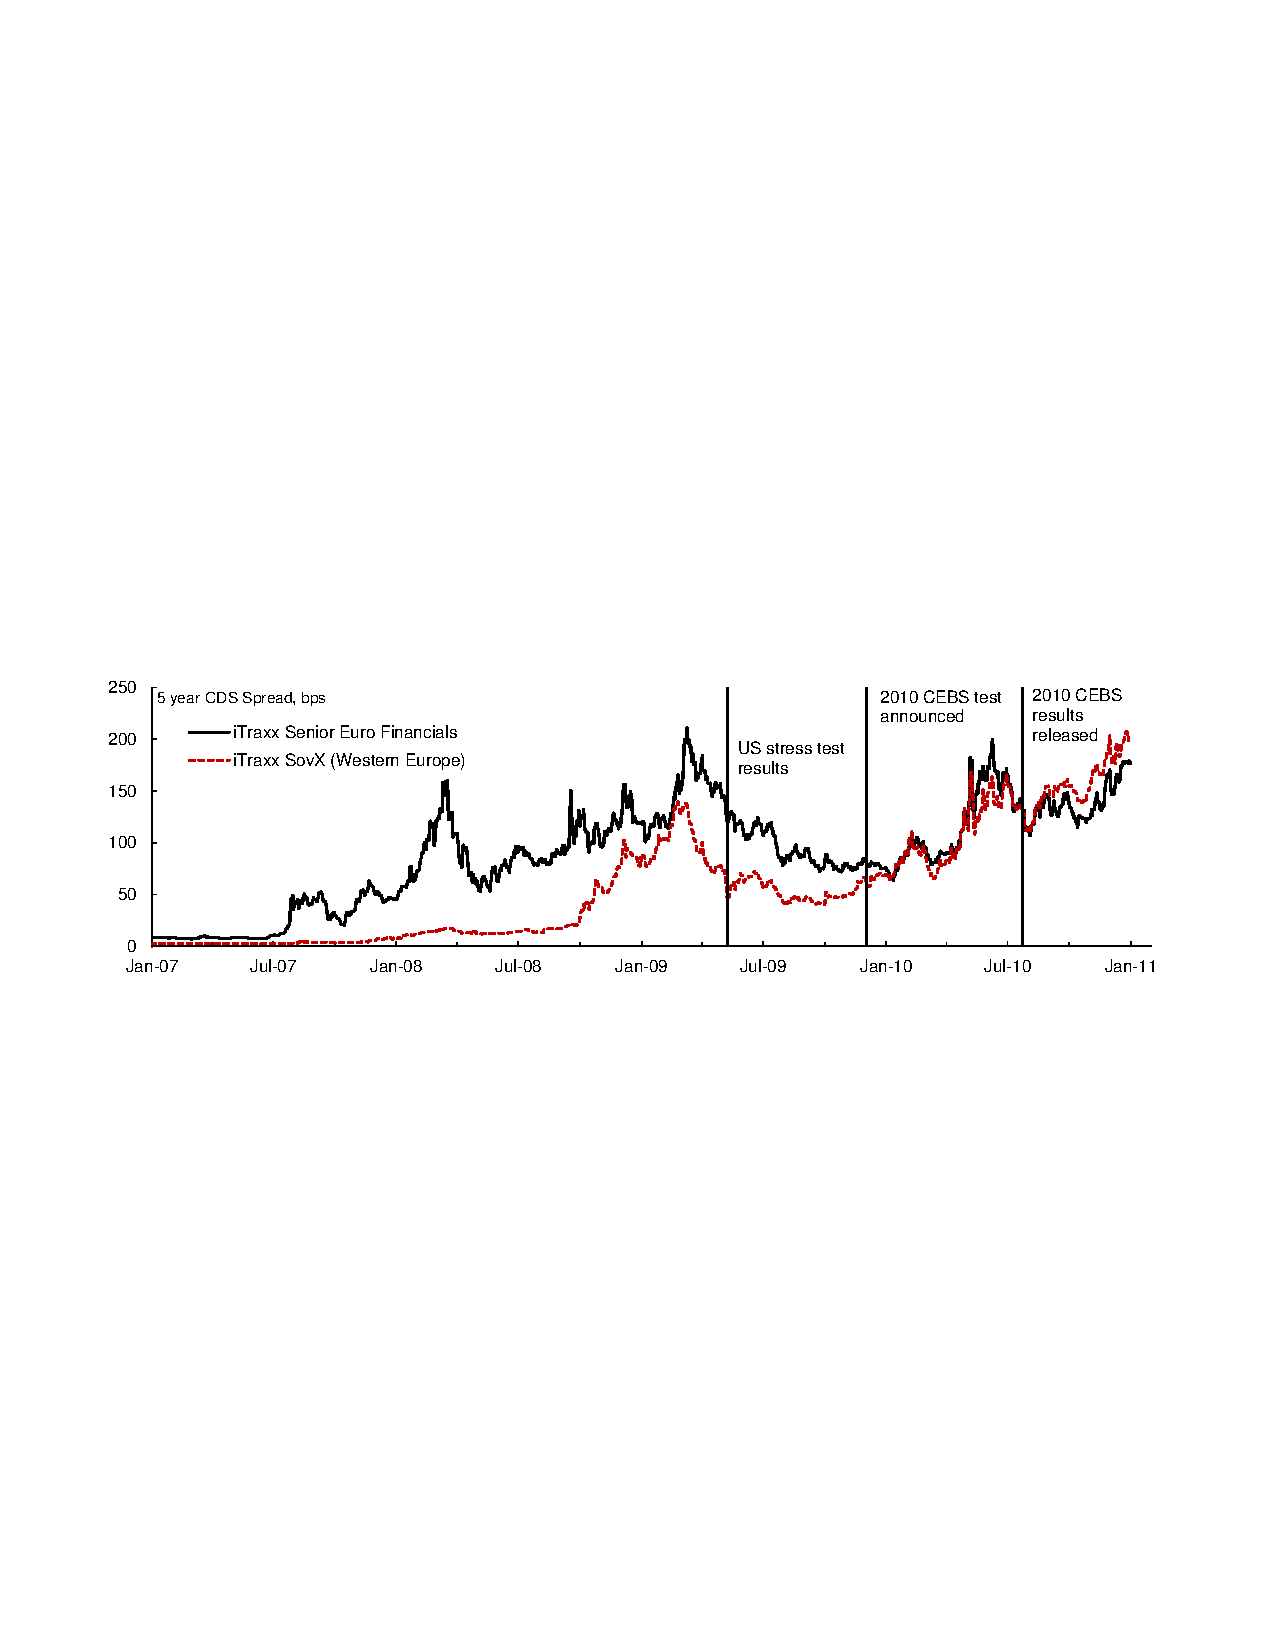
\includegraphics[width=\textwidth]{Chart.pdf}
\raggedright
\textit{\footnotesize Source: Bloomberg, Markit.}
\end{figure}

\begin{figure}[h]
\caption{Real Estate Price Deterioration}\label{figure2}
\centering
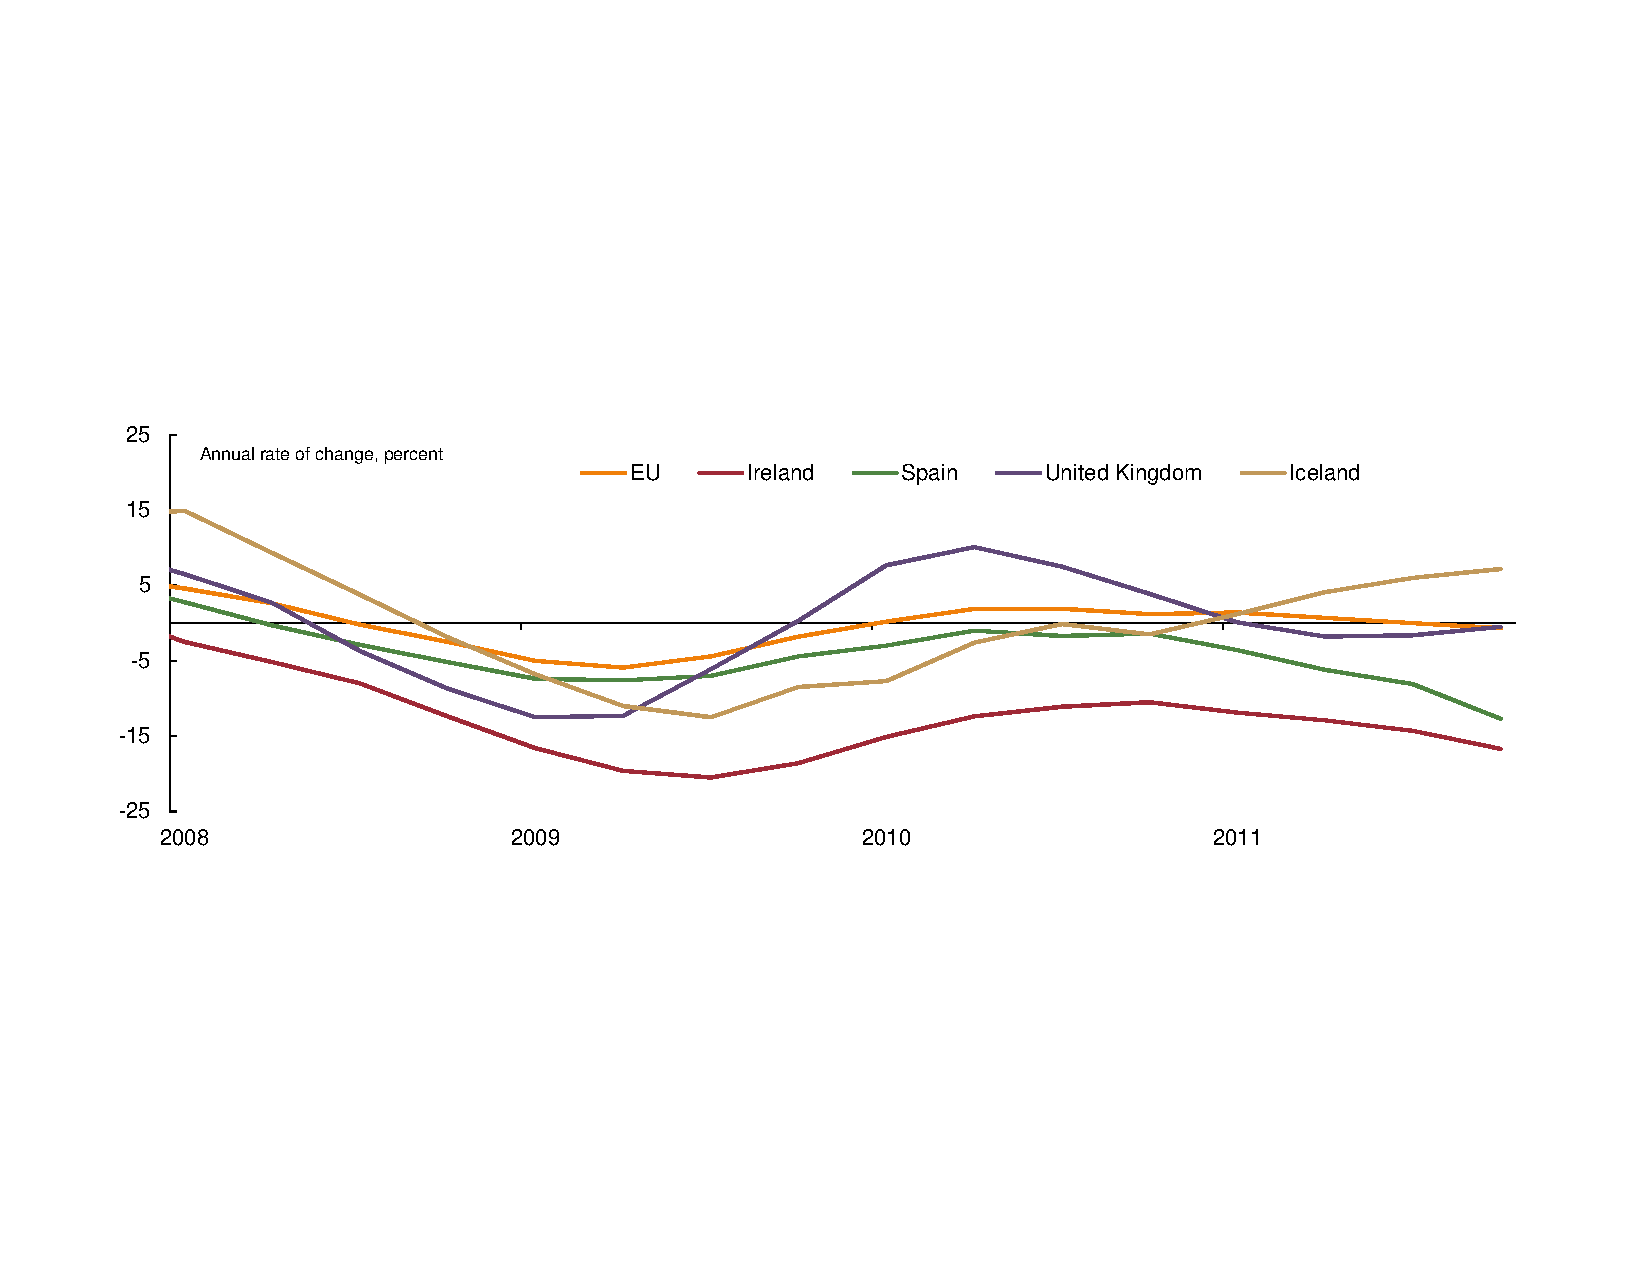
\includegraphics[width=\textwidth]{realestate.pdf}
\raggedright
\textit{\footnotesize Source: Eurostat.}
\end{figure}

Further, real estate prices continued to slide across the EU, as can be seen in Figure~\label{figure2}. Spain, Iceland, and Ireland real estate was falling rapidly, down 4.4\%, 13\% and 19\% respectively.

Finally, the test was announced amid malaise that EU banks had not taken the losses that UK and US banks were compelled to do, in part because of more stringent stress tests in the US and UK, but also due to accounting changes which allowed a shift of distressed assets from trading books to banking books. \citep{Sunderji}. Although the CEBS had concluded a stress test in 2009, with results announced in October 2009 \citep{CEBSOctober2009}, significant uncertainty remained surrounding specific banks' exposures to sovereign debt, and especially to peripheral sovereign debt.\footnote{The peripheral states include Greece, Spain, Ireland, Portugal and Cyprus.} The 2009 test was not received well by markets due to three main reasons: (1) the test's results were only announced via a three page press release describing CEBS' presentation of results to ECOFIN, (2) the methodology was not released, and (3) no bank-by-bank details were published. As a result, investors broadly assumed the worst for all banks and increased funding costs for all banks. The 2010 CEBS test sought to address this concern by providing more clarity regarding bank-specific exposures, aiming to affect the same improvement in public sentiment that accompanied the US's comparable 2009 stress tests. \citep{Goldman}.

\subsection{Program Description}

Unlike the SCAP, CEBS did not publish a detailed methodology before publishing results. However, CEBS published highly detailed (more so than SCAP) methodology documentation simultaneously as the results of the test were released. \citep{Methodology}.

\paragraph{Coverage} The test included 91 European banks from 20 EU member states accounting for 65\% of the total assets in the European banking sector. The test was performed on the highest level of consolidation for the banks involved and also included subsidiaries and branches of European banks operating across the EU and in countries outside Europe. CEBS designed the sample to cover at least half of each Member State's banking market, and as a result there were 7 Member States with a market more than half covered by a subsidiary of a bank already included in the sample. \citep{Methodology}.

\paragraph{Scenarios}

Similar to the US SCAP, CEBS designed the stress test as a set of ``what if'' scenarios rather than forecasts. The test included two scenarios -- a benchmark and adverse scenario -- and then subjected the adverse shock to a sovereign risk shock. The test did not address liquidity risks, but rather focused on market and credit risks. The EC's Interim Forecast in February 2010 and the EU Commission Autumn 2009 forecast set the benchmark forecasts, ``with several adaptations to reflect recent macro-economic developments in a number of countries.'' The adverse scenario was based on ECB estimates. Combined, these forecasts provided estimates for GDP, unemployment and the path of interest rates for each EU Member state, the US and the rest of the world. Table~\ref{design} provides the key parameters used in the test. CEBS and participating national supervisors provided additional parameters ``outside of the narrative of the macro-economic scenarios'' from the ECB and EU Commission, ``notably the evolution of real estate prices.'' Broadly, the macro backdrop used in the test called for a mild recoUK in the benchmark scenarios and double-dip recession in the adverse scenario.


\begin{figure}[h]
\caption{Test Design}\label{design}
\noindent
\makebox[\textwidth]{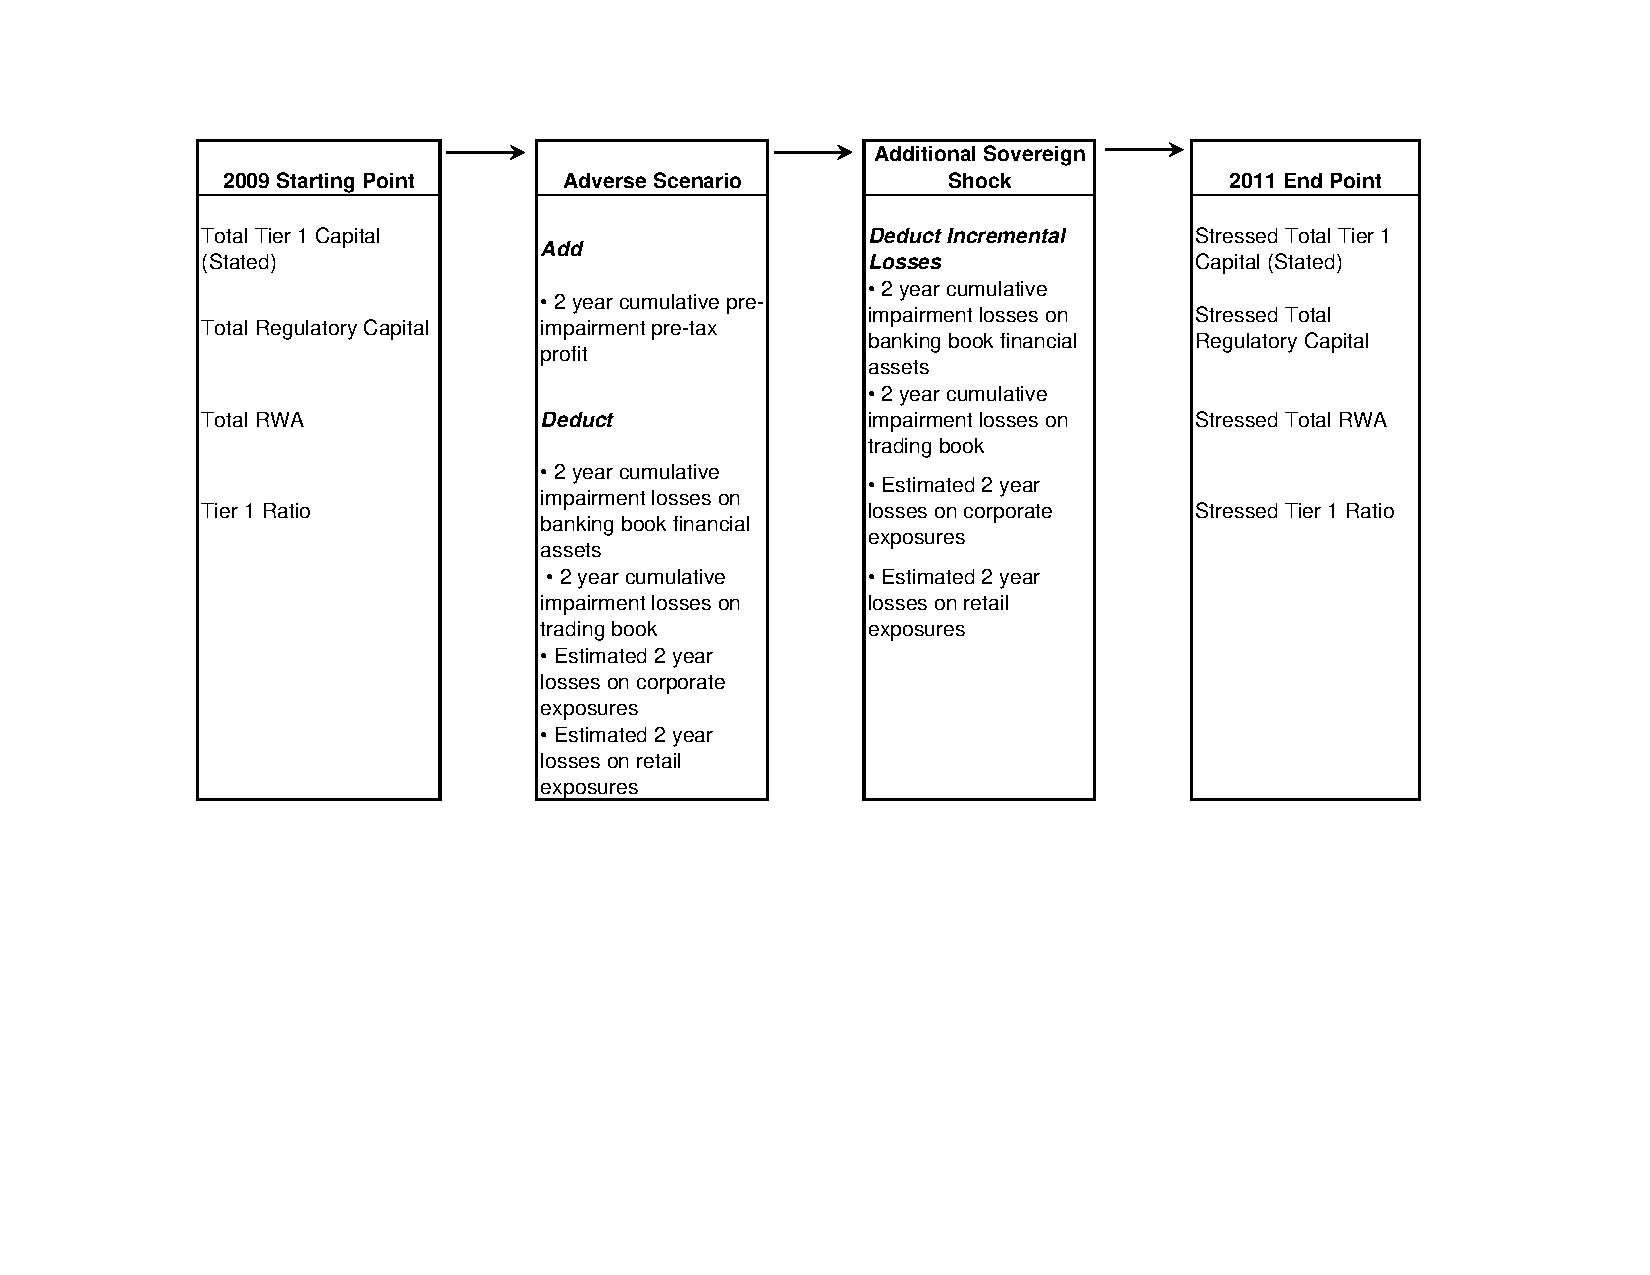
\includegraphics[scale=.70]{flowchart.pdf}}%

\textit{\footnotesize Source: \citet{Deutsche}.}
\end{figure}

\begin{table}[h]
\setlength\LTleft\fill
\setlength\LTright{0pt}
\begin{longtable}[l]{@{\extracolsep{\fill}}@{}ll@{}ll@{}}
\caption{Economic Scenarios}\label{figure3}\\
\toprule
~ & 2010 & 2011 \tabularnewline
\midrule
\endhead
\textbf{Real GDP} & ~ & ~\tabularnewline
EU27 Benchmark & 1.0 & 1.7 \tabularnewline
EU27 Adverse & 0.0 & -0.4\tabularnewline
~ & ~ & ~\tabularnewline
Euro Area Benchmark & 0.7 & 1.5 \tabularnewline
Euro Area Adverse & -0.2 & -0.6\tabularnewline
~ & ~ & ~\tabularnewline
US Benchmark & 2.2 & 2.0 \tabularnewline
US Adverse & 1.5 & 0.6\tabularnewline

~ & ~ & ~\tabularnewline
\textbf{Civilian Unemployment Rate} & ~ & ~\tabularnewline
EU27 Benchmark & 9.8 & 9.7 \tabularnewline
EU27 Adverse & 10.5 & 11.0 \tabularnewline
~ & ~ & ~\tabularnewline
Euro Area Benchmark & 10.7 & 10.9 \tabularnewline
Euro Area Adverse & 10.8 & 11.5\tabularnewline
~ & ~ & ~\tabularnewline
US Benchmark & 10.0 & 10.2 \tabularnewline
US Adverse & 10.2 & 11.1 \tabularnewline

\bottomrule
\multicolumn{3}{l}{\footnotesize Note: GDP calculated year over year; unemployment as a share of labor force.} \tabularnewline
\multicolumn{3}{l}{\footnotesize Source: \citet{Methodology}.} \tabularnewline
\end{longtable}

\end{table}


Further, the adverse shock included an upward shift in the yield curve due to a continuation of the European Sovereign Debt Crisis, at levels similar to those seen at the trough in May 2009. The upward shift can be decomposed into two effects: first, a common upward shift in the yield curve was applied for each country in the EU of 125 basis points for 3 month rates and 75 basis points for 10 year rates at the end of 2011. Second, a country specific upward shift was added on top of the EU-wide shift to account for varying market perceptions of fiscal positions across the EU Member states. These haircuts, shown in Table~\ref{haircuts}, were then applied to each bank's trading book.\footnote{The decision to not impose haircuts on the more opaque banking books proved to be a controversial decision, and is discussed later under the Key Decisions section. However, because the test focused on regulatory capital, some felt it was reasonable to exclude the banking book as losses in hold-to-maturity (HTM) books are typically excluded from regulatory capital.}

\newpage

\begin{table}[htbp]
\setlength\LTleft\fill
\setlength\LTright{0pt}
\begin{longtable}[l]{@{\extracolsep{\fill}}@{}ll@{}}
\caption{Sovereign Debt Valuation Haircuts}\label{haircuts}\\
\toprule
Country & Haircut Value (\%) \tabularnewline
\midrule
\endhead
Greece & 23.1 \tabularnewline
Portugal & 14.1 \tabularnewline
Ireland & 12.8 \tabularnewline
Poland & 12.3 \tabularnewline
Spain & 12.0 \tabularnewline
Czech Republic & 11.4 \tabularnewline
UK & 10.2 \tabularnewline
Italy & 7.4 \tabularnewline
Belgium & 6.9 \tabularnewline
Luxembourg & 6.9 \tabularnewline
Cyprus & 6.7 \tabularnewline
Sweden & 6.7 \tabularnewline
Malta & 6.4 \tabularnewline
Finland & 6.1 \tabularnewline
France & 6.0 \tabularnewline
Austria & 5.6 \tabularnewline
The Netherlands & 5.2 \tabularnewline
Denmark & 5.2 \tabularnewline
Slovakia & 5 \tabularnewline
Germany & 4.7 \tabularnewline
Slovenia & 4.2 \tabularnewline
\bottomrule
Other non-euro area EU & 11.8 \tabularnewline
EU Average & 8.5 \tabularnewline
\bottomrule

\multicolumn{2}{l}{\footnotesize Source: \citet{Methodology}.} \tabularnewline
\end{longtable}

\end{table}


\begin{table}[htbp]
\setlength\LTleft\fill
\setlength\LTright{0pt}
\begin{longtable}[l]{@{\extracolsep{\fill}}@{}ll@{}ll@{}ll@{}}
\caption{5-Year Government Bond Yields in 2011}\label{rates}\\
\toprule
Country & Benchmark\,\, & Adverse & Country-Specific Shock (bps) \tabularnewline
\midrule
\endhead
Austria & 3 & 4.04 & 29 \tabularnewline
Belgium & 3.23 & 4.47 & 49 \tabularnewline
Finland & 3.16 & 4.16 & 25 \tabularnewline
France & 2.94 & 3.92 & 24 \tabularnewline
Germany & 2.74 & 3.49 & 0 \tabularnewline
Greece & 6.28 & 13.87 & 685 \tabularnewline
ireland & 3.28 & 5.62 & 158 \tabularnewline
Italy & 3.19 & 4.8 & 86 \tabularnewline
Netherlands & 2.87 & 3.82 & 20 \tabularnewline
Portugal & 3.96 & 7.4 & 268 \tabularnewline
Spain & 3.61 & 5.75 & 142 \tabularnewline
UK & 4.02 & 5.07 & 30 \tabularnewline

\bottomrule

\multicolumn{4}{l}{\footnotesize Source: \citet{Methodology} and \citet{SG}.} \tabularnewline
\end{longtable}

\end{table}

\paragraph{Key Common Assumptions}

The test assumed ``zero growth'' in the evolution of exposures for market and credit risks over the two year test horizon. Importantly, any public support or management actions (capital issuance or divestment) announced before July 1, 2010 were included in the tests. These measures were included as CEBS assumed sovereigns would continue to provide support to banking institutions well past the two year test horizon which was consistent with the EU's insistence that no sovereign would be allowed to fail. \citep{Alloway}.

Securitized positions under the adverse scenario were assumed to have a four notch decline in the external credit rating over two years, thereby increasing risk-weighted assets (and a direct decrease of regulatory capital). Available-for-sale (AFS) equity exposures were subjected to a 19\% haircut over the two year test horizon in the benchmark, and 36\% in the adverse.\footnote{``Other exposures in the AFS portfolios (i.e. bonds and loans) have been tested along with other credit exposures in the banking book.''} \citep{Methodology}.

\paragraph{Hurdle rate}

The hurdle rate -- the rate at which banks below it would ``fail'' the test -- was set at 6\% of Tier 1 capital. This is the same rate used in the SCAP, although the SCAP also examined capital requirements to maintain a 4\% Tier 1 Common capital ratio.

\subsection{Outcomes}

\paragraph{Aggregate Results} In the adverse scenario, 7 banks failed (of 91) with a cumulative shortfall in Tier1 capital of \euro{3.4} billion. Figure~\ref{tier1outcome} shows the evolution of Tier 1 ratios in the benchmark, adverse, and adverse with sovereign shock scenarios. The banks that failed (e.g. were under the 6\% hurdle rate) are listed in Table~\ref{figure4}, and include five Spanish banks, one German bank, and one Greek bank. In the adverse scenario, aggregate Tier 1 capital would fall from 10.3\% to 9.2\% by the end of 2011.

\newpage

\begin{figure}[h]
\caption{Aggregate Tier 1 Capital by Scenario}\label{tier1outcome}
\noindent
\makebox[\textwidth]{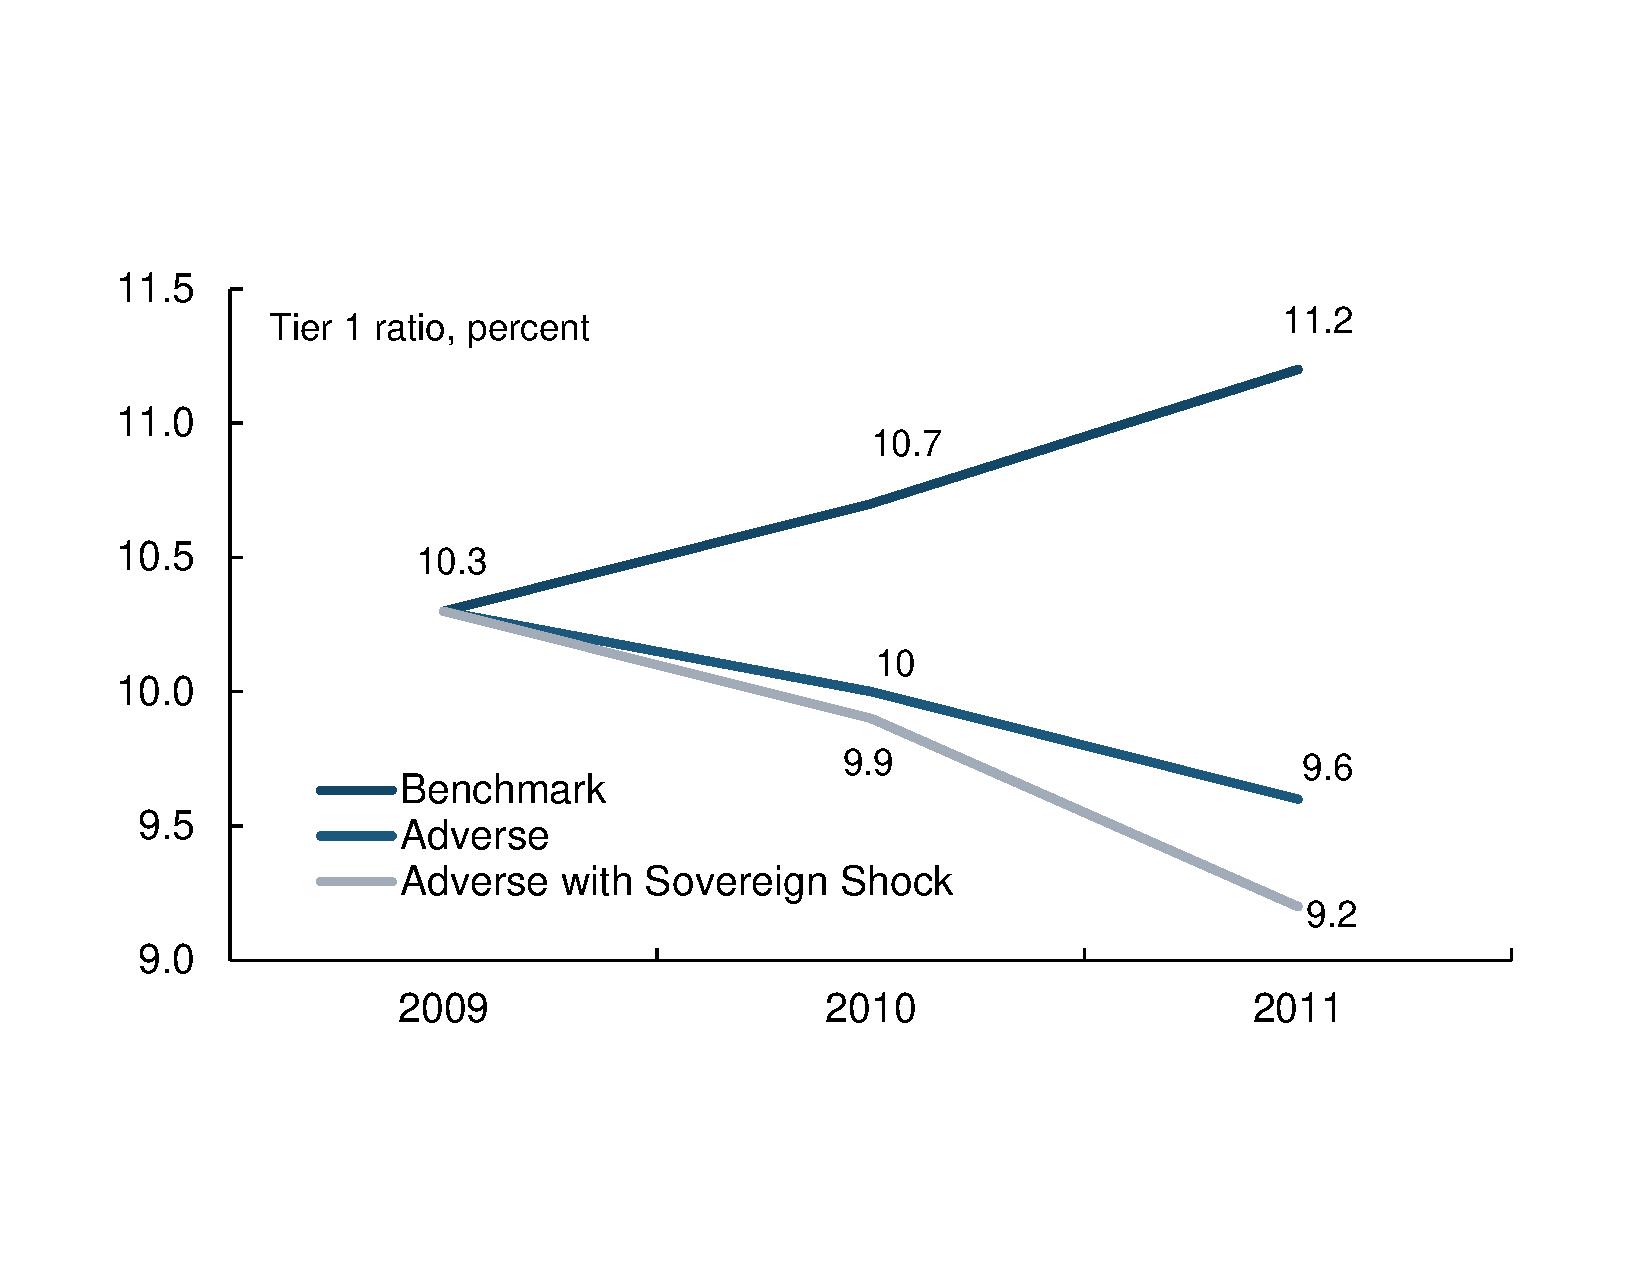
\includegraphics[scale=.50]{tier1outcome.pdf}}%

\textit{\footnotesize Source: \citet{Methodology}.}
\end{figure}


\begin{table}[!htbp]
\setlength\LTleft\fill
\setlength\LTright{0pt}
\begin{longtable}[l]{@{\extracolsep{\fill}}@{}ll@{}ll@{}@{}}
\caption{Banks Below Hurdle Rate}\label{figure4}\\
\toprule
Bank & Country & Tier 1 Capital(\%) & Shortfall (\euro{ millions})\tabularnewline
\midrule
\endhead
Unnim & Spain & 4.5 & 270 \tabularnewline
Diada & Spain & 3.9 & 1,032 \tabularnewline
Espiga & Spain & 5.6 & 127 \tabularnewline
Banca C\'{i}vica & Spain & 4.7 & 406 \tabularnewline
Cajasur & Spain & 4.3 & 208 \tabularnewline
Hypo Real Estate & Germany & 4.7 & 1,245 \tabularnewline
ATEBank & Greece & 4.4 & 243 \tabularnewline
Total & & & 3,531 \tabularnewline
\bottomrule
\multicolumn{4}{l}{\footnotesize Note: Capital ratio is capital stressed under adverse scenario and sovereign shock.} \tabularnewline
\multicolumn{4}{l}{\footnotesize Source: \citet{Methodology}.} \tabularnewline
\end{longtable}
\end{table}

Public support was a key component of the test results. The results note:

\begin{quote}
It should be noted that the maturity of government support measures extended to banking institutions in the sample goes way beyond the two-year time horizon of the exercise. As such, government support form an integral and stable part of the Tier 1 capital ratios of the banks in question. It is not expected that any withdrawal of government support measures could take place without appropriate substitution by private funding sources, where relevant... The aggregate results suggest a rather strong resilience for the EU banking
system as a whole and may appear reassuring for the banks in the exercise,
although it should be emphasized that this outcome is partly due to the
continued reliance on government support for a number of institutions.
\end{quote}

Of the 91 banks in the sample. 20 banks benefited from asset guarantees of some form, and 38 banks benefited from \euro{197} billion of aggregate capital from public sources provided before July 1, 2010 accounting for 14\% of aggregate Tier 1 capital. Therefore, government assistance accounted for 1.2\% of aggregate Tier 1 capital.

The test calculated an estimated \euro{472.8} billion in impairments losses under the adverse scenario with sovereign shock, as well as \euro{38.9} billion in losses in the trading book. Aggregate losses in the EU banking system tested totaled \euro{565.9} billion. Two-year cumulative loss rates for commercial loans was 4.4\%, 2.1\% for retail loans under the adverse scenario.

\paragraph{Market Reception} Market response was mixed. The interbank market reached one-year highs after the results were released, but other price action was muted: Bund futures lost about 3-4 bps in 10 years in the hours after publication. Although the specific methodology was unknown before the results were published, the methodology was in-line with expectations due to a series of leaks from national supervisors in the preceding weeks. The level of disclosure -- the publishing of bank-by-bank sovereign bond holdings -- was a positive surprise, but commentators felt the test lacked credibility in some aspects. Key areas of concern are discussed in Section~\ref{keydesign}. The publication led to so-called ``tiering'' of banks, where market participants used the large amount of data disclosed and subjected each bank to a ``market-realistic stress scenario'' which was more stringent and also included exposures in the banking book. \citep{Nedialkov}

\section{Key Design Decisions}\label{keydesign}

\subsection{27 national supervisors, CEBS, the EU Commission, and the ECB worked together on the test.}

Stress tests were conducted by national supervisory authorities, but were subject to central coordinating guidelines given by CEBS and the ECB with input from the national supervisors. This led to ``some differences in the way the macro-economic scenarios [were] translated into the risk parameters and in the actual application of the reference parameters provided by the ECB,'' but capitalized on national supervisors knowledge of local institutions size, complexity, and sophistication of risk management techniques. This allowed national supervisors to tailor the actual conduct of the exercise to the type of institution: smaller, simpler institutions were subjected to a simplified while more complex, cross-border institutions were tested with bottom-up estimates.

Test results were ``peer reviewed'' -- especially when results relied upon tests run directly by the banks -- where national supervisors met with CEBS representatives in an effort to maintain overall consistency between bank results. National supervisors discussed the results of the tests with banks themselves who occasionally challenged the results before submission to CEBS. \citep{Methodology}

\subsection{The test covered 65\% of banking assets.}

The 2009 CEBS test covered the 26 major cross-border banking institutions in Europe, and the 2010 test expanded this group to include 65 banking groups for a total of 91 banks in all. Combined, the 91 banks had total assets of more than \euro{30} trillion at year end 2009, and accounted for 65\% of the assets in the EU banking system. As mentioned before, the sample of banks was selected so that at least 50\% of each member state's banking system was accounted for.

CEBS was careful to note that, because of the large sample, there was nontrivial heterogeneity between firms. Although the banks represented a diverse set business models, risk profiles and sizes, CEBS was ``confidence that the sample is representative enough to provide a good proxy of the overall resilience of the EU banking sector.'' \citep{Methodology}.

\subsection{Supervisors published the methodology of the stress test and its results at a very detailed level.}

CEBS published the results, and most importantly bank-specific sovereign exposures and the distribution of exposures in banking compared to trading books. This data was made public for all banks except a few German banks which had either supplied exposures to peripheral sovereigns previously (Deutsche Bank) or had been nationalized by the German government already. A key value to the test was not in its estimate of the capital shortfall in Tier 1 funding -- this was subject to a variety of malleable assumptions about sovereign haircuts, sovereign default, forecast assumptions, and public support -- rather the key value was in the transparency it brought about.This largely offset the criticism of CEBS' decision to not stress banking books: the published data allowed market participants to replicate their own preferred stress methodology across both the trading and banking book. Compared to the SCAP disclosures, the 2010 CEBS test provided less detailed information. SCAP provided loss rates across major assets classes (credit cards, commercial real estate, first-lien mortgages and so on) whereas CEBS provided firm specific details on only overall retail and corporate losses.

\subsection{Banks were required to pass a 6\% Tier 1 hurdle rate.}

CEBS directly addressed the choice to use Tier 1 rather than core Tier 1 capital ratios, deciding on the former because CEBS had ``a harmonised and precise legal definition of the components of Tier 1 capital, which is available to absorb losses and maintain a bank as a going concern.'' Further, as the harmonization of core Tier 1 was part of the ongoing G20 reform agenda, ``[u]se of a such a measure... would not have facilitated direct comparison of results across countries.'' \citep{QA}.

The 6\% Tier 1 capital hurdle was more lax than some expected, rather than 6\% Core Tier 1, especially given that government hybrid securities accounted for roughly 1.5 \% of Tier 1 capital. \citep{Gonzalez}. 31 banks were on the margin with between 6 and 8\% capital ratios, and many of the banks with the most public support were also receiving support from the weakest sovereigns, particularly in Greece, Spain and Ireland. If the hurdle rate was 8\% the capital shortfall would have been \euro{27} billion and an additional 31 banks would fail. Moreover, were CEBS to disallow government hybrid securities from the Tier 1 capital ratio, the capital shortfall could rise above \euro{100} billion. \citep{Spick}.

\subsection{Pre-provision profits in the adverse scenario were just 6\% below 2009 levels.}

In the adverse scenario, impairment losses amount to \euro{473} billion and \euro{522} billion with the sovereign shock. This is almost entirely offset by pre-provision revenue of \euro{507} over the two years, compared to \euro{270} billion in profits for the 91 banks in 2009. Thus, the adverse scenario forecast revenues just 6\% below 2009 levels for the 2 year horizon. Some banks forecast greater pre-provision revenue in the adverse scenario than actual 2009 numbers. \citep{Deutsche}.\footnote{This is likely caused by some banks annualizing the high revenues in 2010Q1.} Compared to the fall in pre-provision revenue of roughly 33\% from 2007 to 2009, many felt forecasts for revenues were too optimistic. \citep{Samuels}.

\subsection{The sovereign shock did not include a sovereign default.}

The sovereign shock did not account for a sovereign default, but rather stressed trading books with country-specific haircuts. For example, the sovereign shock included a 23\% haircut on Greek debt, much smaller than would be expected in the case of a Greek default.\footnote{For example, the Greek 3.7\% July 2015 issue traded at 93.34 at year end 2009 and at 72.395 in July 2010, making a 22.4\% decline since year end 2009. The sovereign shock accounted for a 23.1\% haircut on Greek debt from year end 2009, thus representing a shock of an additional 0.7\% from July 2010 actual. The shock was more stringent for Portugal, Ireland, Spain and Italy; respectively testing a leg down of (respectively) 8.6\%, 10.1\%, 10.8\% and 8\%. \citep{Danske}.} CEBS justified the exclusion of sovereign default as the creation of the European Financial Stability Facility (EFSF) in early 2010 indicated policy was to not allow a sovereign default:

\begin{quote}
The setting up of the European Financial Stability Facility (EFSF) and the related commitment of all participating member States provides reassurance that the default of a member State will not occur, which implies that impairment losses on sovereign exposures in the available for sale and held-to-maturity in the banking book cannot be factored into the exercise. \citep{QA}.
\end{quote}


\subsection{There was no explicit capital backstop.}

Public support was included in the test only insofar as the support had been provided by July 2010, and there was no explicit capital backstop for those which failed. This is a significant departure from the precedent set by the SCAP: whereas the SCAP provided a public backstop, via the Capital Assistance Program\footnote{The Capital Assistance Program was ultimately not used by any of the 19 firms tested.} to bank holding companies failing the SCAP should they be unable to raise capital privately, the 2010 CEBS tests had no analogous program. The lack of a capital backstop raises questions about the rigor of a stress test as supervisors have an incentive to whitewash concerns as there is no backup should large capital shortfalls be revealed. Instead, CEBS provided guidance that banks that fail or almost fail may be asked to increase their capital buffers:

\begin{quote}
Banks whose capital ratios decline and move towards the threshold value set up for this stress, will as we always do in such situation, be subject to closer supervisory scrutiny and more intrusive supervision. If deemed necessary, the national supervisor will ask the bank’s management to develop a plan to improve the situation, including potentially, a plan to increase capital buffers, which will be subsequently assessed by the national supervisory authority.
\end{quote}

CEBS provided guidance on the process in which a bank could receive public support. State aid exceeding 2\% of risk weighted assets was subject to European Commission scrutiny, as Article 107(1) of the Treaty on the Functioning of the European Union prohibits State aid which disrupts a level playing field in the internal market. However, the Commission can approve state aid either in the form of a generalized scheme or on a case-by-case basis. CEBS also highlighted that the European Commission could provide scrutiny in a very short time period -- overnight or over weekends -- should it be necessary. These rapid response approvals were often temporary ``in order to safeguard financial stability.'' \citep{QA}.

In deciding whether approve the provision of state aid to a bank, the Commission asks (1) whether the assistance is necessary because the bank is ``fundamentally sound'' but requires assistance due to market turmoil, in which case a bank would only be required to submit a viability plan which states its ability to be viable over the long-term independent of state aid, or (2) whether the assistance is necessary because of more fundamental problems with the bank -- it is found to be ``non-fundamentally sound -- in which case the bank would be required to submit comprehensive restructuring plan. \citep{QA}.

Further, should a Member State need to support a bank but be unable to raise funds themselves, the European Financial Stability Mechanism (EFSM) or the European Financial Stability Facility (EFSF) could be used to indirectly provide support to the bank via the Member State, as both the EFSM and EFSF do not have the legal authority to directly provide financial support to the banking sector. \citep{QA}.


\subsection{Sovereign stresses applied to trading books and banking books differently.}

Sovereign debt haircuts were applied to trading books but not directly to the banking books (i.e. available-for-sale and held-to-maturity securities). The banking book was not directly affected as in a strict sense that the test focused on regulatory capital and losses in the held-to-maturity book are generally not counted within regulatory capital. The banking book was stressed in the follow manner: the haircuts for valuation losses in the trading book ``induce a change in the probability of default and loss-given-default for the household and corporate sector, given that higher long-term government bond yields also imply higher borrowing costs for the private sector, which in term imply higher probability of defaults and loss-given-defaults for the non-sovereign exposures.'' Therefore, losses in the sovereign shock scenario are unrelated to sovereign exposures in the banking book, but rather the losses stemming from higher borrowing costs due to higher sovereign spreads. \citep{Samuels}. However, the disclosures provided sufficient level of detail of bank-specific exposures (except for a handful of German banks) that it was easy for market participants to apply a similar stress to the banking book.

Compared to SCAP, CEBS used a more aggressive calculation: SCAP used the more conservative standard that examined ``on whether... it is more-likely-than-not that firms will be required to sell the security before recovery of its cost base.'' Were this the case, firms were required to recognize an other-than-temporary-impairment, with the loss equal to the difference between the amortized cost basis and the fair value of the investment. \citep{SCAPResults}.

\subsection{The tests assumed a continuation of existing public support.}

The test included public support in the form of pre-July 2010 capital injections (either via equity or hybrid instruments) and also government guarantees of bank assets. 20 banks benefited from asset guarantees and 38 banks benefited from \euro{197} billion of public capital. This increased aggregate Tier 1 capital by 1.2\%. Public support was included as the support had ``a useful life extending beyond the horizon of the exercise.'' One analyst noted: ``This might be consistent with the European Union's comments that no sovereign will be allowed to fail, but... it just doesn't seem quite right...[T]he banks with significant government support... are often located in some of the weaker European countries.'' \citep{Alloway} Specifically, Greek banks benefited from \euro{9.4} billion in capital injections, Spanish cajas received funding from the Fund for Orderly Bank Restructuring (FROB), and Irish banks had received public capital as well.

\citet{Alloway} also notes that CEBS inclusion of hybrid government securities was at odds with rating agencies decision to exclude the same from Tier 1 capital after the European Commission shifted away reliance on hybrid capital.\footnote{See \citet{Fitch}. Hybrid capital, with both equity and debt like characteristics, and is included in banks' Tier 1 and 2 capital under Basel rules at the time of the 2010 CEBS test. Hybrid capital was favored by many banks, notably Deutsche Bank, Standard Chartered and Credit Agricole, as it was both cheap to issue and non-dilutive. At year end 2008, hybrid capital accounted for roughly 28\% of European banks' capital base. \citep{Alloway2}.}

\subsection{Forecast scenarios were produced by national supervisors and the adverse scenario represented a ``double dip'' recession.}

The primary forecast relied upon a 3\% decline in EU wide GDP, compared to a fall of 2.9\% in the SCAP. CEBS loss assumptions fit a mild recession, unlike very stringent SCAP loss assumptions.\footnote{For example, SCAP used a 2 year commercial loan loss rate of 9\%, compared to CEBS 4.4\%.} When looking at the country-specific unemployment forecasts, the SCAP called for a 1.4\% increase in unemployment, greater than any the increase for any country in the CEBS test. Figure~\ref{unemployment} shows the country-specific unemployment rates. There was also meaningful variation across countries in terms of their real estate price forecasts, as can be seen in Figure~\ref{REforecast}.


\begin{figure}[h]
\caption{$\Delta$ Unemployment in Adverse Scenario}\label{unemployment}
\centering
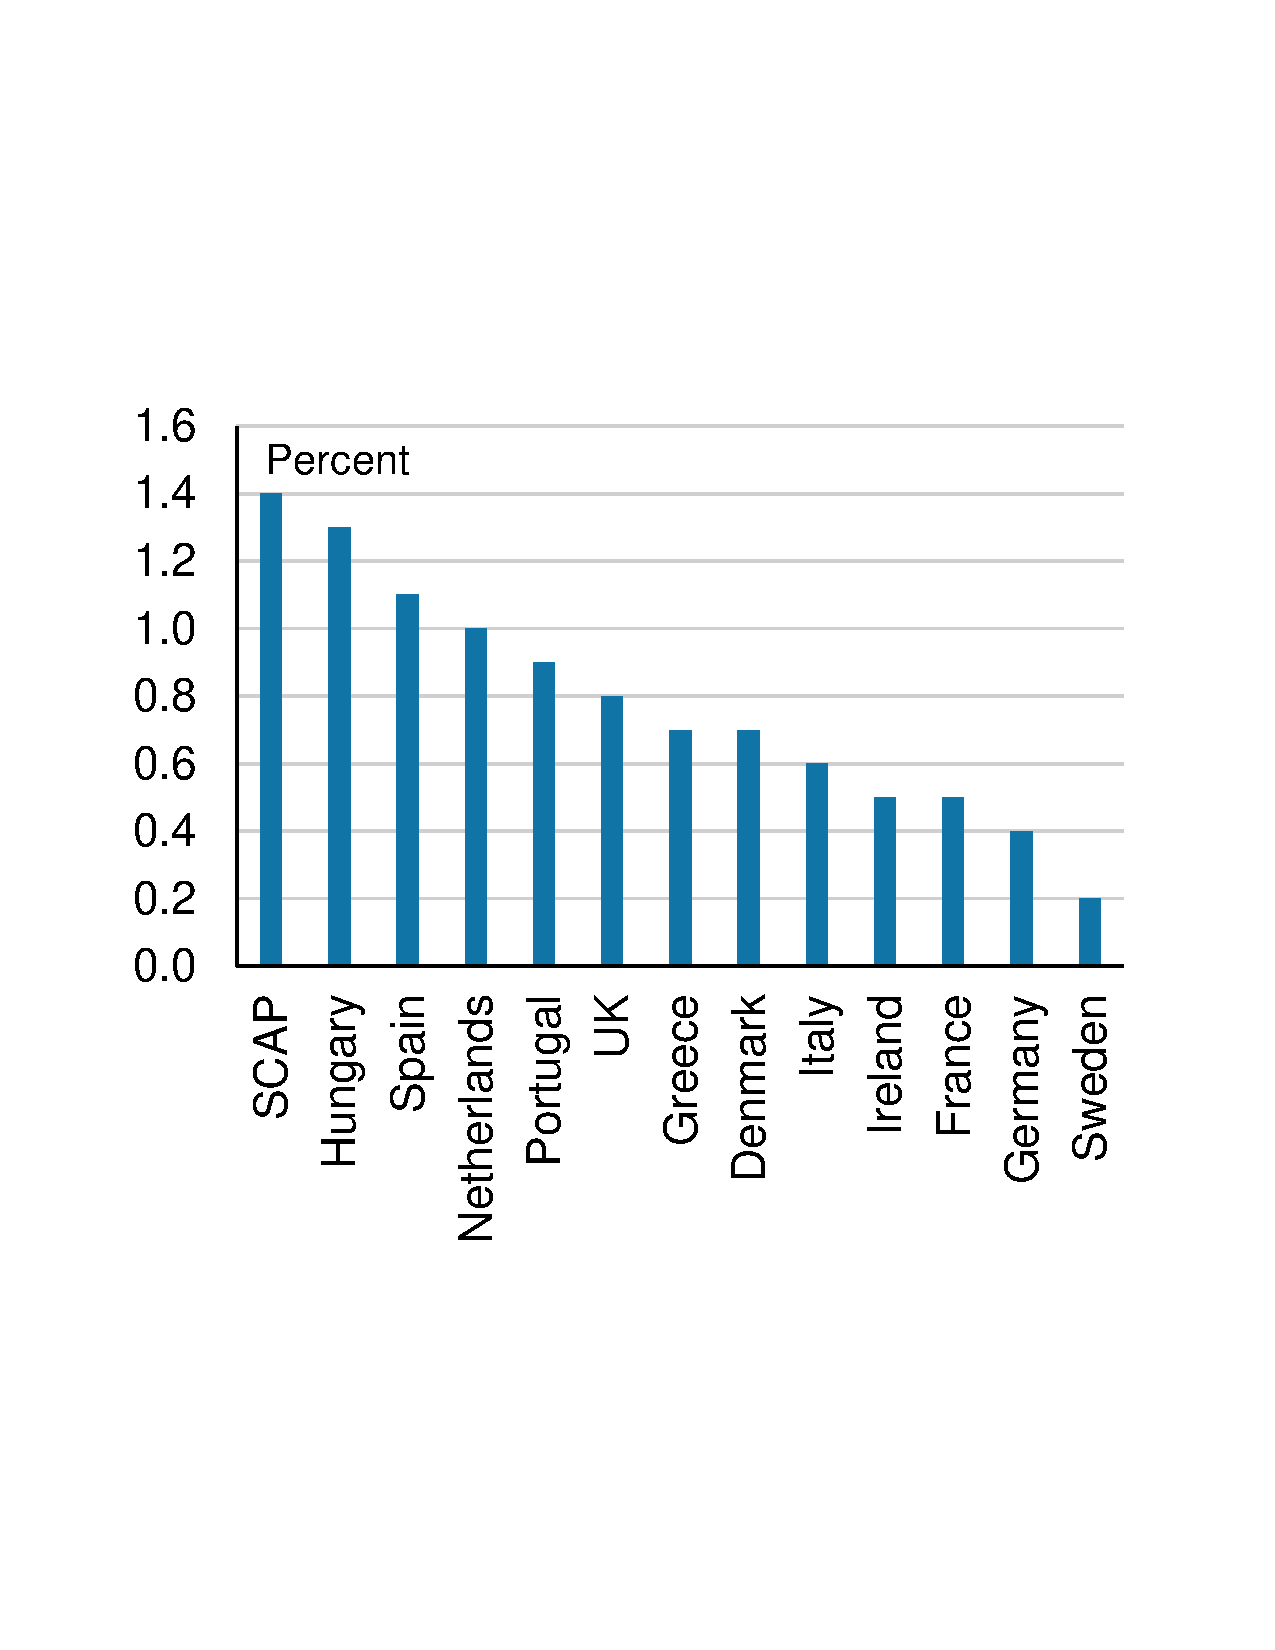
\includegraphics[width=.45\textwidth]{unemployment.pdf}

\raggedright
\textit{\footnotesize Source: \citet{Methodology}.}
\end{figure}

\begin{figure}[h]
\caption{Cumulative decline in real estate prices in Adverse Scenario}\label{REforecast}
\centering
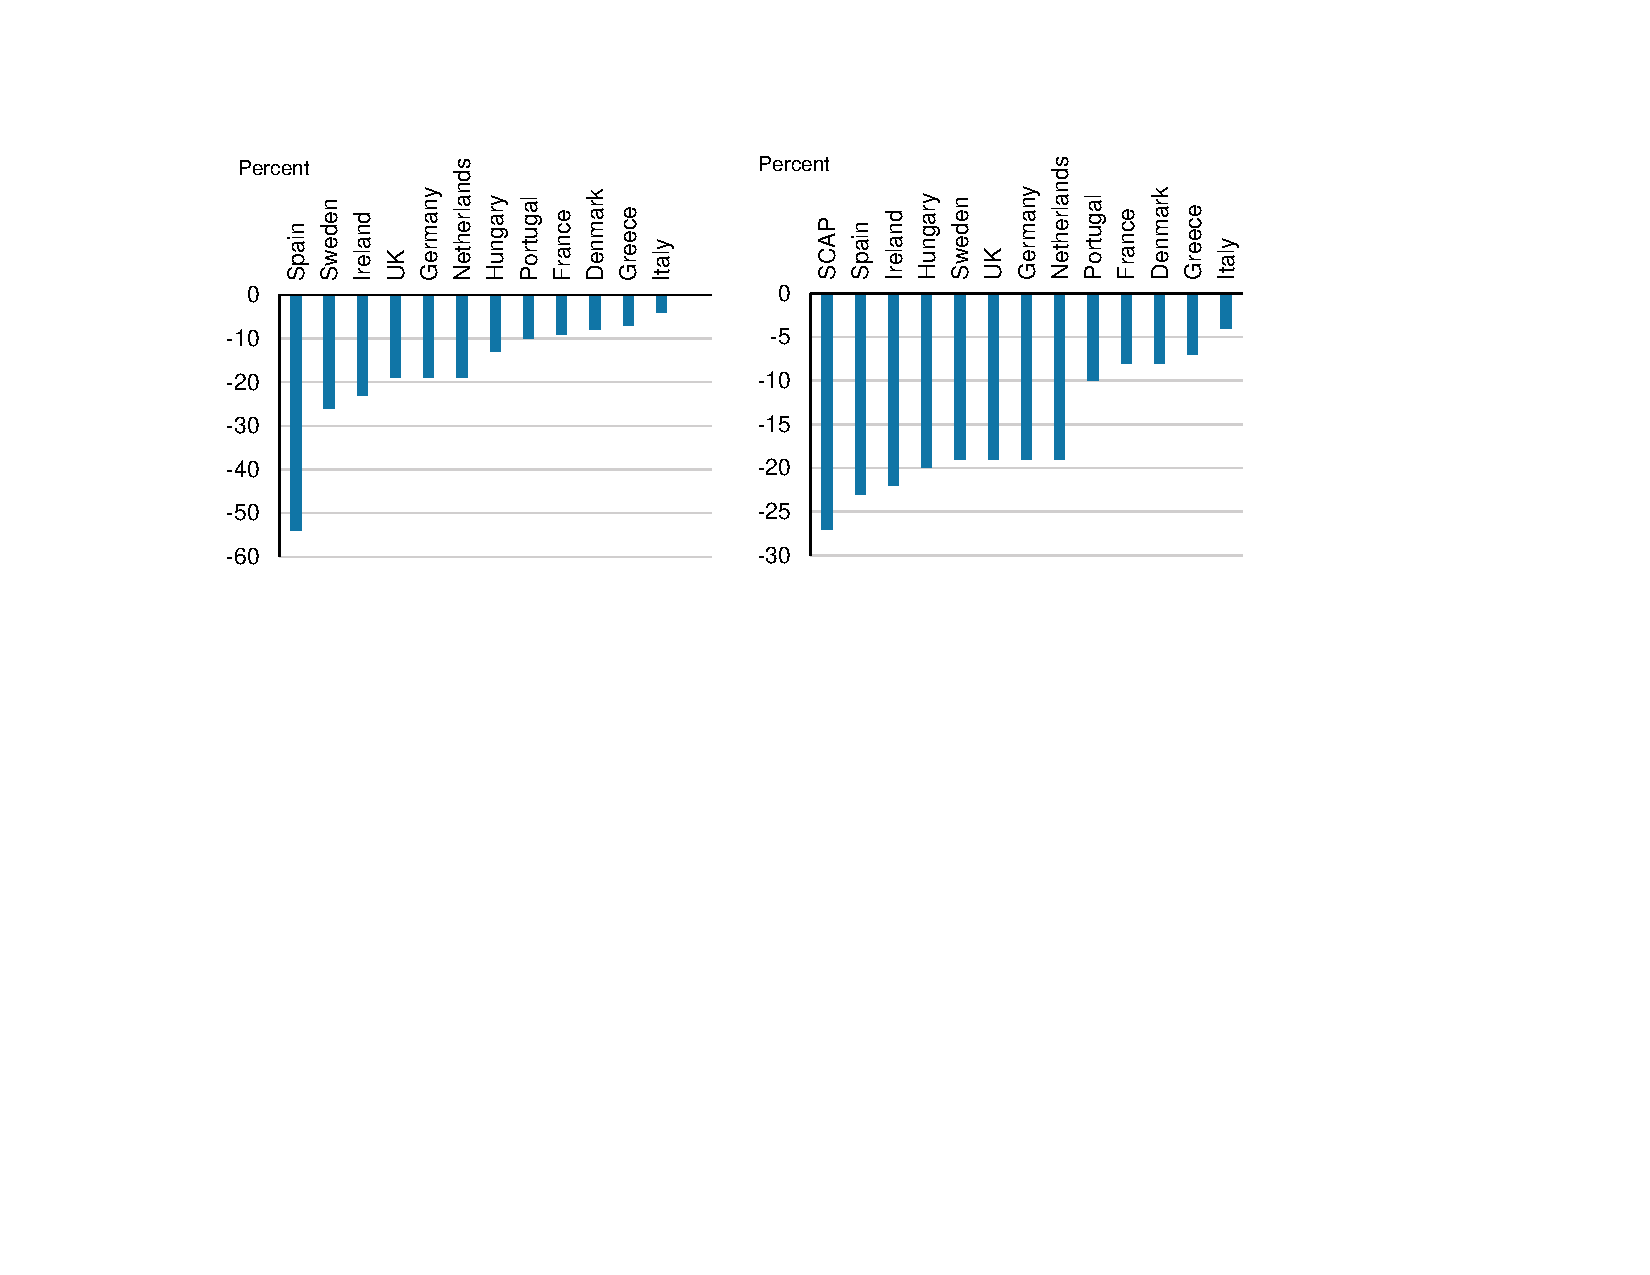
\includegraphics[width=\textwidth]{REforecast.pdf}
\raggedright
\textit{\footnotesize Source: \citet{Methodology} and \citet{SCAPResults}.}
\end{figure}

\section{Evaluation}

A natural comparison with the 2010 CEBS test is the US SCAP test in 2009. CEBS directly addressed the comparison. CEBS noted a handful of similarities between the two: (1) a focus on credit risk, (2) two macroeconomic scenarios, (3) a two year time horizon and (4) roughly the same proportion of assets in the banking system. \citep{QA}.

CEBS noted four significant differences. Most importantly, the purpose between the two diverges. SCAP was ``directly link to determining the individual capital needs of banks,'' whereas the CEBS test aimed ``to provide policy information for the assessment of the individual Member States of the resilience of the EU banking sector as a whole and of the banks participating in the exercise.'' Second, the US test was less complex in the sense that CEBS tested 91 banks (rather than SCAP's 19) and coordinated across 27 national supervisors as well as CEBS and the ECB (rather than SCAP's 3). Third, the CEBS test emphasized sovereign exposures. And finally, US supervisors conducted SCAP specifically ``in the context of a major government intervention and in order to gage the magnitude of the needs,'' whereas CEBS performed the test after many public interventions. \citep{QA}.

\citet{Posen} describe a key disadvantage to the CEBS test in the lack of a general banking union, causing a ``collective-action failure.'' National supervisors, aware of issues in their own country's banks, were incentivized to post-pone addressing their own problems until other national supervisors did the same.

\begin{quote}
For each national authority, the incentive was thus to pretend that the extent of problem loans was not only exaggerated (while actually allowing them to increase), but also that the worst problems were outside of their own territorial remit (while going soft on supervision at home). This became all too apparent in the inadequate stress tests whose results were announced in September 2009, July 2010, and July 2011. Banks like Dexia were given a clean bill of health, only to collapse a few months later. Self-defeating supervisory behavior is hardly unique to euro area bank supervisors, but the escalation of such reality denial in the face of market panic and bank-sovereign doom loops in 2010–11 was the result of banking nationalism.
\end{quote}

\citet{OECD} emphasize the importance of the 2010 stress test ignoring sovereign exposures in the banking book. Due to the difficulty of fiscal consolidation during slow growth in Europe at the time of the tests, market participants could not assign zero probability to the risk of debt restructuring. They find 83\% of the banks' sovereign exposure at year end 2009 was in the banking book.

\citet{Engle} study CEBS 2010 test, along with four other stress tests conducted in the US and EU which provided bank level disclosures, and make three findings. First, they find that the estimated losses on the balance sheet by stress tests and market-based assessments are similar, and are representative of actual losses. Second, required capitalization of those tested is low compared to what is implied by market data. The contradiction of the first and second finding can be explained by the ``reliance on regulatory risk weights in stress tests in determining required levels of capital once stress-test losses are taken into account.'' Therefore, they conclude, that risk weights provide ``perverse incentives'' for firms to take on more exposure to lower risk-weight assets leaving the banking system undercapitalized, which they find to be particularly true during the European sovereign debt crisis.

\citet{Schuermann2011} describes market reaction to the stress test results as ``benign'' despite the limited disclosure (compared to the SCAP). However, he notes, the credibility of the test suffered significantly after when Ireland turned to the EU and IMF for support in November 2010, four months after the 2010 test passed the included Irish banks with no capital shortfall. To bolster the credibility of its own stress test in March 2011, the Central Bank of Ireland engaged Blackrock to conduct the test and provided loss rates across a variety of asset classes -- residential mortgages, corporate loans, small and medium enterprise loans, commercial real estate and others.\footnote{\citet{Ireland} provides the results of Ireland's stress test in March 2011.} Blackrock found a capital shortfall of \euro{24} billion. Due to this unprecedented level of transparency and the credibility of the independent outside advisers sovereign and bank spreads tightened in Ireland. \citet{Schuermann2011} concludes, ``[t]he stakes for the 2011 European stress test... had risen substantially.''

\citet{Schuermann2016} finds that ``rigorous use of independent models'' in stress tests is an important component for credibility, and one that the EU-wide tests in 2010 and 2011 lacked. As both the 2010 test inadequately stressed the Irish banking sector and the 2011 test inadequately stressed the Spanish banking sector (where a subsequent test found a capital shortfall of \euro{57} billion)``it seems hard to imagine how a supervisor could effectively evaluate the impact of scenarios on bank balance sheets (and income statements) without their building own models.''

Other researchers note that the disclosure of bank-specific data can materially impact the credibility of the supervisor. \citet{Itay} consider a scenario in which stress test results provide no new information. In this scenario, the act of disclosure affects the supervisors' credibility as ```regulators could be held accountable as their supervisory approach--whether in terms of how credible the tests are and/or what supervisory actions would be taken with regards to banks that fail the test--would be subject to greater scrutiny and discussion by outsiders.'' \citet{Itay} suggests the SCAP was particularly successful, not due to the information contained in the disclosures, but rather because the Federal Reserve had announced what the bar for passing was, what would happen to firms that did not pass, and what supervisors would do with firms that did not pass before the results were announced. ``Conversely, it is widely believed that [the 2010 CEBS test] lacked such credibility and did little to enhance the reputation of the superiors.''

\citet{Candelon} perform event study tests and find that the CEBS tests in 2010 had a positive and significant impact on the value of stressed banks, and no significant effect on nonstressed EU banks. Further, among their sample of stress tests, the 2010 CEBS tests was the only test which had a positive effect on the value of stressed banks. They find that increased disclosure does restore confidence in a banking system, but rather that the ``governance challenges that led to insufficient coordination and lack of coordination among EU members to come up with better estimates of sovereign losses and a financial backstop.''

\newpage
\phantomsection

\addcontentsline{toc}{section}{References}

\nocite{*}
\bibliography{\jobname}

\newpage


\section{Appendix A - List of Resources}

\subsection{Summary of Program}

\begin{itemize}
\item
\ul{Questions and Answers: 2010 EU-Wide Stress Testing Exercise}, Committee of European Banking Supervisors, July 23, 2010 -- \emph{CEBS
 document outlining the purpose of the test and highlighting key results.} \url{https://www.ecb.europa.eu/pub/pdf/other/euwidestresstestingexercise-qaen.pdf?860c12759915bf0e3a8cd5486cb595a4}
\end{itemize}

\subsection{Implementation Documents}
\begin{itemize}
\item
\ul{Aggregate Outcome of the 2010 EU Wide Stress Test Exercise Coordinated by CEBS in Cooperation with the ECB}, Committee of European Banking Supervisors, July 23, 2010 -- \emph{CEBS
 document outlining design details and results of the test.} \url{https://www.eba.europa.eu/documents/10180/15938/Summaryreport.pdf/95030af2-7b52-4530-afe1-f067a895d163}
\item
\ul{Summary of the 91 bank-by-bank results, by country}, Committee of European Banking Supervisors, July 23, 2010 -- \emph{CEBS
 document disclosing bank-by-bank data.} \url{https://www.eba.europa.eu/documents/10180/15938/Listofbanksv2.pdf/af7d6849-5882-4f83-82e7-b4ff9a63a112}
\end{itemize}

\subsection{Legal/Regulatory Guidance}

\begin{itemize}
\item
\ul{Treaty on the Functioning of the European Union -- Chapter 1: Rules on competition - Section 2: Aids granted by States - Article 107 (ex Article 87 TEC)}, -- \emph{Portion of the TFEU which outlines how state aid may be approved by the European Commission.} \url{http://eur-lex.europa.eu/legal-content/EN/ALL/?uri=CELEX\%3A12008E107}
\item
\ul{Fitch Downgrades Lloyds, RBS, ING, Other EU Banks' Hybrids on Increased Risk of Coupon Deferral}, Fitch Ratings, August 20, 2009 -- \emph{Fitch Rating's justification for downgrading various EU banks due to their reliance on hybrid capital.} \url{http://ftalphaville.ft.com//2009/08/20/67906/hybrid-debt-attack-for-real-from-fitch/}
\end{itemize}

\subsection{Press Releases/Announcements}

\begin{itemize}
\item
\ul{CEBS Press Release on the Results of the 2009 EU-Wide Stress Testing Exercise}, CEBS, October 1, 2009-- \emph{Press release which
 announces the results of the 2009 EU-wide stress test.} \url{https://www.eba.europa.eu/documents/10180/15977/CEBS-2009-180-Annex-2-\%28Press-release-from-CEBS\%29.pdf}
\item
\ul{Press Release: 2981st Council Meeting, Economic and Financial Affairs}, Council of the European Union, December 2, 2009 -- \emph{Press release
 announcing the 2010 EU-Wide stress test.} \url{https://www.consilium.europa.eu/uedocs/cms_data/docs/pressdata/en/ecofin/111706.pdf}
\item
\ul{CEBS Press Release on the Results of the 2010 EU-Wide Stress Testing Exercise}, CEBS, July 23, 2010-- \emph{Press release which
 announces the results of the 2010 EU-wide stress test.} \url{https://www.eba.europa.eu/documents/10180/15938/CEBSPressReleasev2.pdf/4a5b185f-43bf-4e4d-b1de-c50c7e656b87}
\end{itemize}

\subsection{Media Stories}

\begin{itemize}
\item
\ul{Stress Test's Sovereign Support = Senseless}, Tracy Alloway, Financial Times, July 26,
 2010 -- \emph{Article discussing and criticizing the public support included in the tests.} \url{http://ftalphaville.ft.com/2010/07/26/296871/stress-tests-sovereign-support-senseless/}
\item
\ul{Tear Down This Hybrid Capital Wall}, Tracy Alloway, Financial Times, September 9, 2009 -- \emph{Article discussing the use of hybrid capital.} \url{http://ftalphaville.ft.com//2009/09/09/70611/tear-down-this-hybrid-capital-wall/}

\end{itemize}

\subsection{Key Academic Papers}

\begin{itemize}
\item
\ul{Macrofinancial Stress Testing -- Principles and Practices},
 IMF, 2012 -- \emph{Paper discussing the various forms of stress tests and, most importantly, provides a comparison of crisis management stress tests including the SCAP and other similar European stress tests.} \url{https://www.imf.org/external/np/pp/eng/2012/082212.pdf}
\item
\ul{Testing Macroprudential Stress Tests: The Risk of Regulatory Risk Weights},
Acharya, Engle and Pierret, 2014-- \emph{Paper discussing the accuracy of various stress tests and how risk weights can negatively affect banks' recapitalization.} \url{http://pages.stern.nyu.edu/~sternfin/vacharya/public_html/pdfs/Testing_Macro_Stress_Tests_March27.pdf}
\item
\ul{The EU Stress Test and Sovereign Debt Exposures},
Wignall-Blundell and Slovik, 2010-- \emph{Paper discussing the location of sovereign exposures across the trading and banking book during the 2010 stress test, as well as governance reasons for the test's credibility.} \url{http://search.proquest.com/docview/1081470338?pq-origsite=gscholar}
\item
\ul{Stress Testing Banks},
Til Schuermann, 2011-- \emph{Paper discussing the how stress test can help the banking system regain trust and the costs and benefits of bank-specific information compared to aggregate information.} \url{http://papers.ssrn.com/sol3/papers.cfm?abstract_id=2041579}
\item
\ul{Stress Testing in Wartime and Peace},
Til Schuermann, 2016-- \emph{Paper discussing the difference between stress tests performed as crisis interventions versus those conducted in normal times.} \url{http://papers.ssrn.com/sol3/Papers.cfm?abstract_id=2735895}
\item
\ul{Should Banks' Stress Test Results be Disclosed? An Analysis of the Costs and Benefits},
Goldstein and Haresh, 2013-- \emph{Paper discussing, among other things, how stress tests can affect a supervisor's credibility.} \url{http://faculty.chicagobooth.edu/Haresh.Sapra/research/docs_RP/stresstests_GS_FTF_Dec_2013.pdf}
\item
\ul{How Did Markets React to Stress Tests?},
Candelon and Sy, 2015-- \emph{Paper providing an event study of various significant stress tests.} \url{https://www.imf.org/external/pubs/ft/wp/2015/wp1575.pdf}

\end{itemize}

\subsection{Reports/Assessments}

\begin{itemize}
\item
\ul{Europe's Half a Banking Union}, Adam Posen and Nicolas Veron, Bruegel, September 19, 2014 -- \emph{Report discussing the importance of a banking union to produce credible stress test results.} \url{http://bruegel.org/2014/09/europes-half-a-banking-union/}
\item
\ul{The Financial Measures Programme Report}, Central Bank of Ireland, March 2011 -- \emph{Central Bank of Ireland's report, produced with outside independent advisers, which stressed the Irish banking system and found significant capital shortfalls despite Irish banks passing the 2010 EU-wide test 8 months earlier.} \url{http://www.centralbank.ie/regulation/industry-sectors/credit-institutions/Documents/The\%20Financial\%20Measures\%20Programme\%20Report.pdf}
\end{itemize}

\section{Appendix B - Road Map}

The following is a list of the key design decisions that will likely have to be made in implementing a program similar to the 2008/9 FSA stress test, a' program intended to assess the capital needs of financial institutions receiving taxpayer support during a period of heightened uncertainty around potential losses in the banking system.

\subsection{Key Questions}

\begin{outline}[enumerate]

\1 Which agency or agencies have the authority and expertise to conduct the stress test?
\2 What is the basis of this authority?
\2 What particular elements/terms must be satisfied to fit within the authority?
\2 After designing, have all required elements been satisfied?
\1 What, if any, capital backstop should be available to firms which undergo the stress test?
\2 Does the existence or lack of a public capital backstop affect market views of the test's credibility?
\2 Is any additional authority required in order to provide a capital backstop?
\2 How can the backstop be structured to compel firms to first raise private capital and use the public capital as a less preferred option?
\2 How long should firms be allowed to seek private capital before turning to the public backstop?
\1 How should a public capital backstop be structured?
\2 What sort of security should the public capital be provided through?
\2 Should economic conditions worsen, can the public capital convert into common equity (at a discount)?
\2 What other constraints will firms using public capital face? (E.g. executive compensation caps, restrictions on common stock dividends, buybacks and cash acquisitions, etc.)
\1 Which firms are included in the stress test?
\2 How many firms can be credibly tested given the testing agency's resources?
\1 How transparent should the test results be? What level of granularity for estimates should be publicly available?
\2 If the issue is sovereign exposures, how should these sovereign exposures be stressed?
\1 How can the regulators ensure the test is viewed as credible?
\2 How should existing public support be incorporated into the test?
\2 What metric or measure should regulators target to assess capital adequacy?
\3 What is the target hurdle rate?
\3 What data on bank holdings and capital adequacy does the testing agency collect as part of its regular bank examination process? Is this data sufficiently granular for the test or will further data need to be collected?
\3 Should the test focus on Tier 1 capital, Tier 1 Common capital, Core Tier 1 capital, tangible common equity, a combination of these or something else?
\4 Should hybrid securities associated with pubic support be included?
\4 For example, should preferred equity, goodwill and intangible assets be included in the equity component?
\4 Should the denominator be based on risk-weighted assets, tangible assets or something else?
\1 Over what time frame is the stress test examining capital adequacy?
\2 Should the stress test measure in-the-moment or measure ``in the stress''?
\1 What economic scenarios are used to stress the firms?
\2 How do you ensure consistency in the forecast parameters across many jurisdictions?
\2 Who produces the scenarios, and at what level of geographic specificity are they produced?
\2 How many economic scenarios are used to stress the firms?
\2 How do these scenarios compare with contemporary private forecasts?

\end{outline}

\subsection{Implementation Steps}

\begin{enumerate}

\item Develop the description of the test, including legal authority, purpose, firm eligibility, a general timeline, et cetera and seek input from industry and other stakeholders.
\item If necessary, seek approval for the program, funding et cetera.
\item If a capital backstop will be used, establish a description of the backstop with legal authority, firms eligible to receive the backstop, the mechanics of the capital injection, et cetera and seek input from industry and other stakeholders. Produce term sheet for the program.
\item Produce economic scenarios with which to stress capital adequacy and distribute it to the tested firms.
\item If firm-level data at a sufficiently granular level is not available from the traditional bank examination processes, collect the relevant data from firms.
\item Draft detailed FAQs and template for published results.
\item Using the provided economic scenarios and bank portfolio data, both supervisors and firms individually produce capital adequacy estimates.
\item Compare supervisors' capital adequacy estimates with firms' own estimates and reconcile differences.
\item If necessary, develop instructions for completing the documentation necessary to participate in the capital back stop.
\item Publicly release stress test results.

\end{enumerate}


\end{document}
